\documentclass{beamer}
%\documentclass[handout]{beamer} % set [handout] as an option to remove /pause breaks

%\setbeameroption{show notes on second screen=right} % Make sure slide position is set to "right" in pympress also, or if using pdfpc, with --notes=right
% Also, comment out the notes to produce slides for archiving, etc.
\usetheme{Berlin}
% There's no McMaster specific template and *THERE SHOULD BE*
% use pympress on the rendered pdf to have things like second screen, notes, etc! Cool!
% EXTREMELY IMPORTANT: if you are *sharing this content over Teams on your Linux laptop*, for instance, do the following:
% Boot Ubuntu
% Select Xorg from login menu (sigh)
% use CHROME to access teams: e.g. google-chrome teams.microsoft.com
% Share the pympress main presentation window using the share tray.
\usepackage{verbatim}
\usepackage{fancyvrb}
\usepackage{tikz}
\usepackage{chemfig}
%\usepackage{mathtools}
\usepackage[version=4]{mhchem}

%title page details:
\title{\LaTeX{} Engineering Grad Society Presentation}
\subtitle{A presentation about \LaTeX{} to the McMaster EGS}
\author{John Fink}
\institute{McMaster University}
\date{July 19th, 2022}


\begin{document}

	\begin{frame}
		\titlepage
	\end{frame}

	\begin{frame}
		Who am I?
		\note{I'm John Fink, Digital Scholarship Librarian at the Mills Library. I am, quite thoroughly, not an engineer or a scientist. I have, embarrassingly enough, a creative writing degree. Through a series of mostly accidents / being in the right place at the right time, most of my working life has been STEM or STEM adjacent, mostly as a systems administrator and now as a research librarian}
	\end{frame}

\begin{frame}
	What can you do with \LaTeX{}?
\end{frame}

\begin{frame}{What can you do with \LaTeX?}
	\begin{itemize}
		\item Scholarly articles
		\pause
		\item Books and book chapters
		\pause
		\item (bibliography support through Bib\TeX)
		\pause
		\item Presentations (like this one!)
		\pause
		\item Resumes/CVs
	\end{itemize}
\end{frame}
		

\begin{frame}
	What is the difference between \textit{word processing} and \textit{typesetting}?
\note{}
\end{frame}

\begin{frame}
	% A fun comparison of word vs. LaTeX here: https://mappingignorance.org/2015/04/06/word-or-latex-typesetting-which-one-is-more-productive-finally-scientifically-assessed/
	Why choose typesetting over (most) word processing?
	\begin{itemize}
		\item The source is \textit{portable} and \textit{versionable}. Anything that can edit text can edit \LaTeX.
		\pause
		\item It is \textit{way} easier to do things like inline formulas ($E=mc^2$), images, and tables.
		\pause
		\item Easy to generate indices, bibliographies, cross references
		\pause 
		\item It allows you to \textit{write} without worrying what the writing \textit{looks like}.
		\pause
		\item \LaTeX{} can produce some \textit{beautiful} output. Even the stock PDF output is pleasant!
		\pause
		\item The documentation for \LaTeX{} is \textbf{vast} (and beautiful, of course) and there's a StackExchange answer for just about anything you'd think to ask.
		\pause
		\item You can generate many document types -- PDFs, ePubs, yes, even Word format -- from \LaTeX source.
	\end{itemize}
	
	\note{Portable as in ascii text. There is simply no other format extant that will guarantee as much interoperability and long-term preservation as straight up text will. It can be version controlled. It can be put anywhere. It will definitely outlast me and probably you.}

\end{frame}

\begin{frame}{And perhaps most importantly...}
	Most STEM specific journals can accept submissions in \LaTeX, and some will \textbf{only} accept submissions in \LaTeX.
\end{frame}

\begin{frame}
	Worry about \textbf{content}, not (or not as much) about \textbf{form}.
\end{frame}


\begin{frame}
	Why choose word processing \textit{over} typesetting?
\end{frame}

\begin{frame}
	\begin{itemize}
		\item Everybody everywhere uses Word.
		\pause
		\item \LaTeX{} is a \textit{programming language}
		\pause
		\item \LaTeX{} final documents have to be compiled (this presentation takes about 7 seconds)
		\pause
		\item Word is \textit{much better} than it used to be re: generating ToCs, using templates, etc.
	\end{itemize}
	\note{Programming language in both the good and bad senses of the term. Good: it's *precise*. It does what you ask it to do. It doesn't surprise you. Bad: OK, there's the *IDE* (or lack thereof), there's the fact if you omit a closing bracket your entire thing will just ... stop working. Programming!!!}
\end{frame}

\begin{frame}
	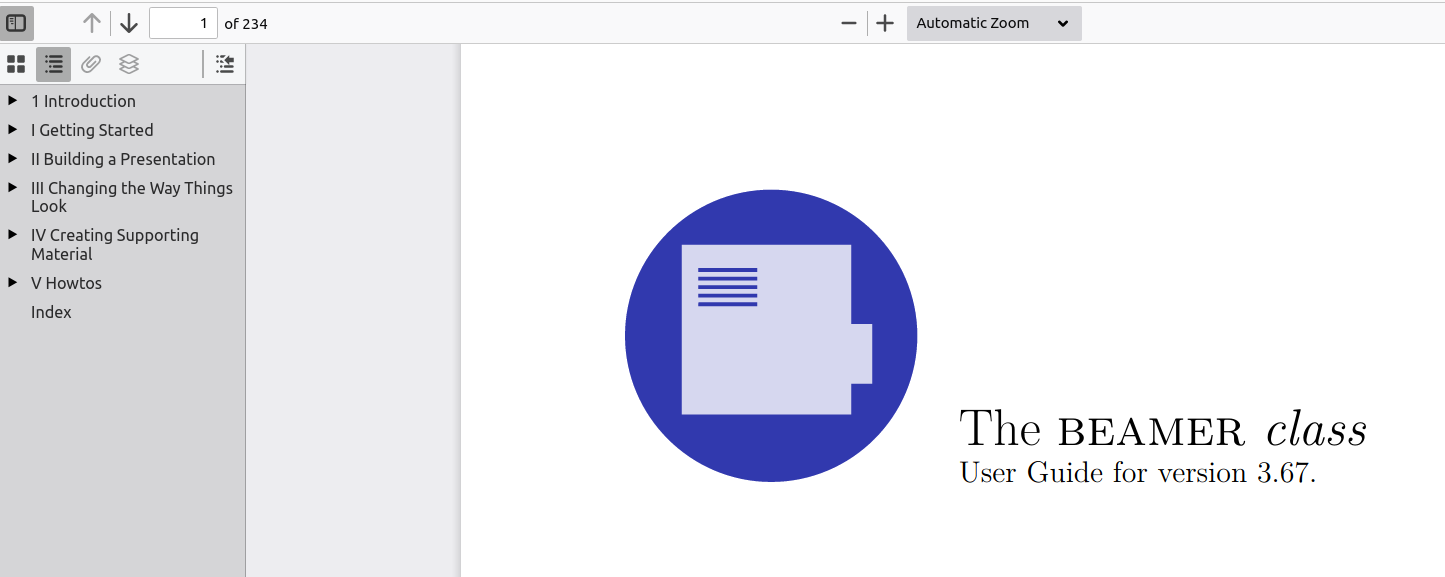
\includegraphics[height=6cm]{beamer-manual}
	\note{This is the manual for Beamer, the document class for slide decks. It's not the full LaTeX manual, it's just for slides. I want to draw your attention to the upper left hand corner -- that's 234 pages. Of manual. Just for slides!}
\end{frame}

\begin{frame}
	What is \LaTeX{}?
\end{frame}

\begin{frame}
	What is... \TeX?
	%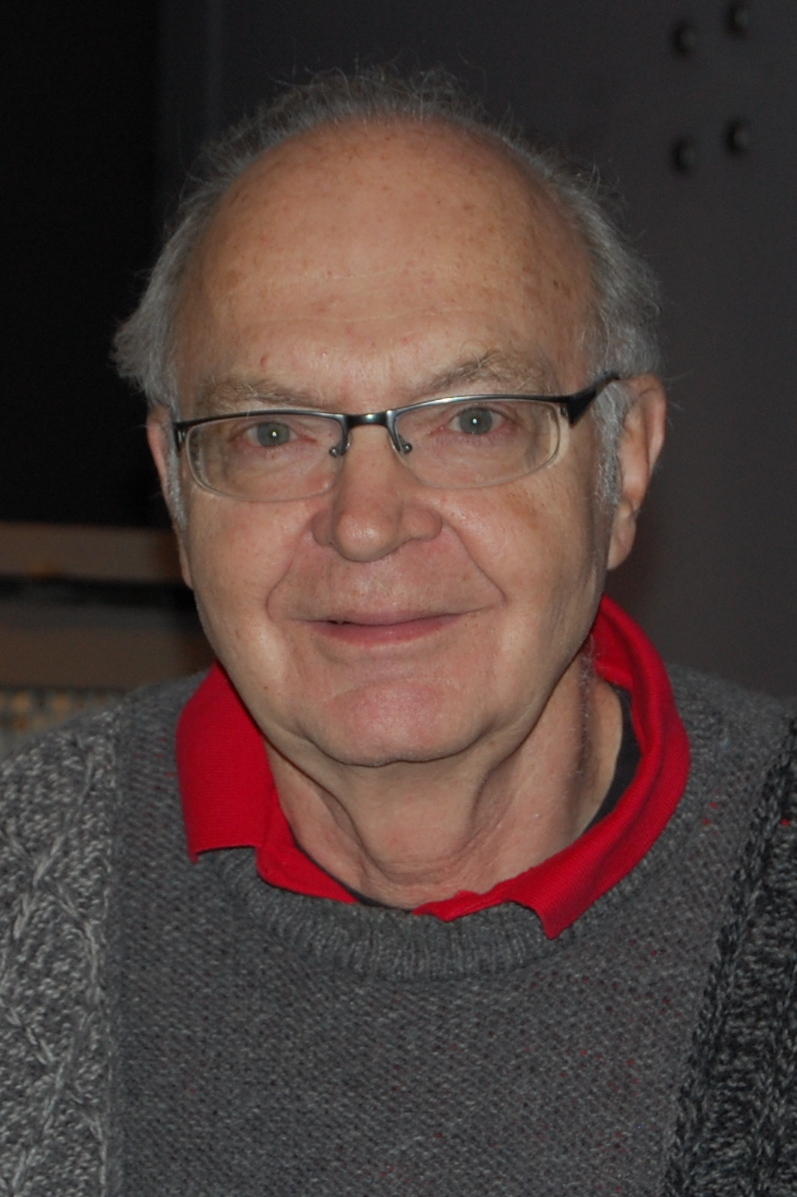
\includegraphics[height=5cm]{knuth}
	\begin{itemize}
		\item Invented by Donald Knuth in 1978.
		\pause
		% below history is from https://tex.stackexchange.com/questions/39442/tex-troff-a-reflection-on-the-history-of-computer-typography#39448
		\item Intended as a replacement for the Unix \textit{troff} command, which by 1978 was apparently a very patchy mess.
		\pause
		\item So rather than make more patches, Knuth developed \TeX.
	\end{itemize}
	\note{wikpedia sez: "is a typesetting system which was designed and written by Donald Knuth[1] and first released in 1978. TeX is a popular means of typesetting complex mathematical formulae; it has been noted as one of the most sophisticated digital typographical systems."}
\end{frame}

\begin{frame}
	So what is \LaTeX?
	\pause
	It's \TeX{} with added sauce:
	\pause
	\begin{itemize}
		\item Optimized for publishing
		\pause
		\item Numbering, cross-referencing
		\pause
		\item Tables and figures
		\pause
		\item Page layout
		\pause
		\item Bibliographies
		
	\end{itemize}
\end{frame}

\begin{frame}
	The \textbf{structure} of a \LaTeX{} document.
	\note{a LaTeX document is *just text*. You can edit it with anything that edits plain text and doesn't mangle it, you can put it in version control, you can copy it anywhere, you can be assured that -- as plain text -- it will probably be viewable, at least as text, for the forseeable future (my lifetime, if not yours at least)}
\end{frame}

\begin{frame}
	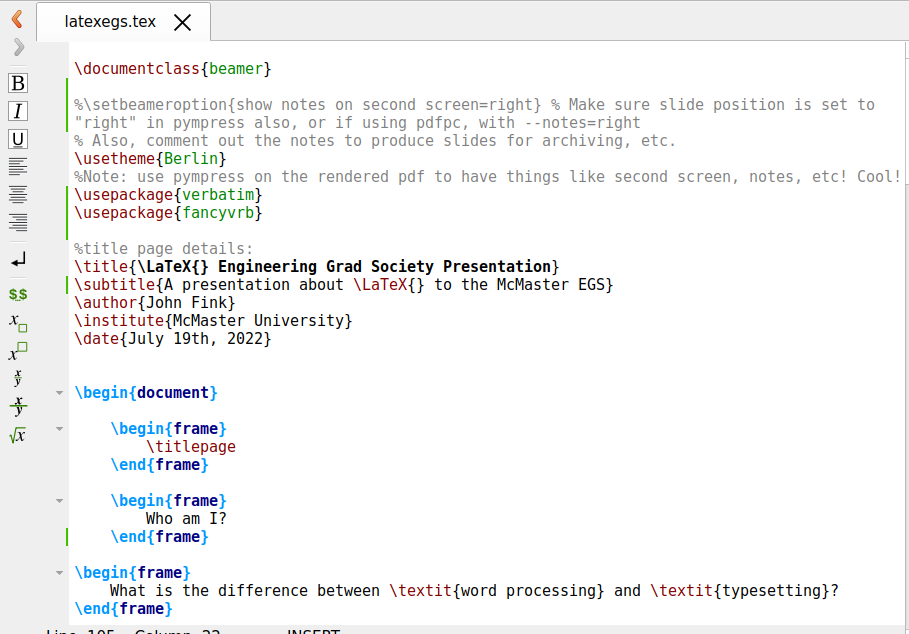
\includegraphics[height=8cm]{latex-structure}
	\note{Let's take a look here. This is the beginning of my slide deck for this very talk -- yup, that's right, you can actually write slides in LaTeX just like any other document. First, you have the preamble -- this sets up your document. Let's go through it, shall we?}
\end{frame}

\begin{frame}[fragile=singleslide]
\begin{Verbatim}
\documentclass{beamer}
\usetheme{Berlin}
\usepackage{verbatim}
\usepackage{fancyvrb}
%comments start with a % sign.
\end{Verbatim}
\note{Beamer includes a lot of packages by default so when you write a paper in LaTeX you might find yourself using way more usepackage statements -- for example, including graphics is not a default package in many LaTeX document classes}.
\end{frame}


\begin{frame}[fragile=singleslide]
	%Verbatim here instead of verbatim as Verbatim is fancyvrb, which I needed for font size changes. Phew!
	\begin{Verbatim}[fontsize=\small]
%title page details:
\title{\LaTeX{} Engineering Grad Society Presentation}
\subtitle{A presentation about \LaTeX{} to the McMaster EGS}
\author{John Fink}
\institute{McMaster University}
\date{July 19th, 2022}
	\end{Verbatim}
	\note{The percent is a comment, of course. Title is title of the presentation -- could be title of a paper or a book, but we're using Beamer, so it's a presentation -- a subtitle, the author, the institute, and the date.}
\end{frame}

\begin{frame}[fragile]
	So just about any \LaTeX{} specific markup will look like:
	\begin{itemize}
		\item A \verb|\| character
		\pause
		\item A \textbf{command}, like \textit{includegraphics}
		\pause
		\item \textbf{options} passed to the command, in \verb|[]|, like \verb|[height=8cm]|
		\pause
		\item The information fed to the command, in \verb|{}|, like \verb|{imagename}|
		\pause
		\item So, the command \verb|\includegraphics[height=8cm]{imagename}| will display the image titled \textit{imagename}, scaled to 8cm height.
	\end{itemize}
	\note{Whoof! A lot to take in. Note that, in LaTeX, at least when you're inserting images, you do not specify an image extension -- e.g., no imagename.png or whatever, just imagename.}
\end{frame}



\begin{frame}
	Drawing in \LaTeX{} with the tikz package
\end{frame}

\begin{frame}[fragile=singleslide]{Drawing in \LaTeX with the tikz package}
\begin{Verbatim}[fontsize=\scriptsize]
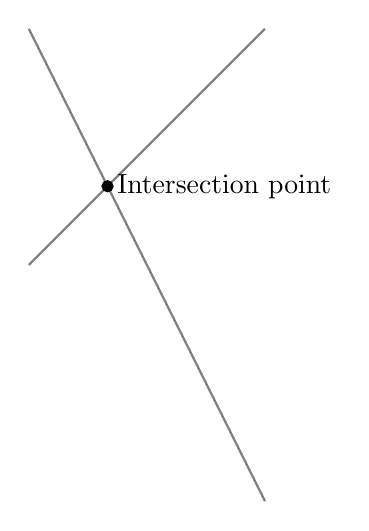
\begin{tikzpicture}
\draw[gray, thick] (-1,2) -- (2,-4);
\draw[gray, thick] (-1,-1) -- (2,2);
\filldraw[black] (0,0) circle (2pt) node[anchor=west]{Intersection point};
\end{tikzpicture}
\end{Verbatim}
\end{frame}

\begin{frame}{Drawing in \LaTeX with the tikz package}
	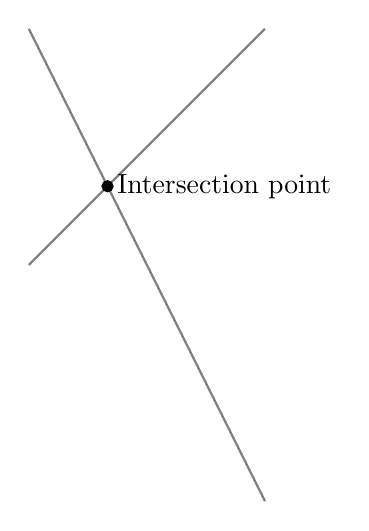
\begin{tikzpicture}
		\draw[gray, thick] (-1,2) -- (2,-4);
		\draw[gray, thick] (-1,-1) -- (2,2);
		\filldraw[black] (0,0) circle (2pt) node[anchor=west]{Intersection point};
	\end{tikzpicture}
\end{frame}	

\begin{frame}[fragile]{Doing Math Stuff in \LaTeX}
	\begin{itemize}
		\item Inline formulas are done with \verb|$..$| or \verb|\..\| or \verb|\begin{math}..\end{math}|
		\item (these are all, as far as I know, identical in use)
		\pause
		\item e.g. the universal law of gravitation: $F=\frac{Gm_1 m_2}{r^2}$.
		\pause
		\item In code: \verb|$F=\frac{Gm_1 m_2}{r^2}$.|
	\end{itemize}
\end{frame}

\begin{frame}[fragile]{Doing Math Stuff in \LaTeX}
	\begin{itemize}
		\item Display mode formulas are done with \verb|\..\|, \verb|\begin{displaymath}..\end{displaymath}|, \verb|\begin{equation}..\end{equation}|
\end{itemize}
\end{frame}
	
\begin{frame}[fragile]
	\begin{equation}
		E=m
	\end{equation}
	\pause
	\begin{Verbatim}
		\begin{equation}
			E=m
		\end{equation}
	\end{Verbatim}
\end{frame}

\begin{frame}{Tables in \LaTeX}
	\begin{tabular}{||l|c|r|p{6cm}||}
		Left & Center & Right & Paragraph \\
		1 & 1 & 1 & Lorem ipsum dolor sit amet, consectetuer adipiscing elit. \\
		12 & 12 & 12 & Ut purus elit, vestibulum ut, placerat ac, adipiscing vitae, felis. \\
		123 & 123 & 123 & Curabitur dictum gravidamauris. \\
	\end{tabular}
\end{frame}

\begin{frame}[fragile]
\begin{Verbatim}
\begin{tabular}{||l|c|r|p{6cm}||}
	Left & Center & Right & Paragraph \\
	1 & 1 & 1 & Lorem ipsum dolor sit amet, consectetuer adipiscing elit. \\
	12 & 12 & 12 & Ut purus elit, vestibulum ut, placerat ac, adipiscing vitae, felis. \\
	123 & 123 & 123 & Curabitur dictum gravidamauris. \\
\end{tabular}
\end{Verbatim}
\end{frame}

%The chemistry stuff is here: https://www.overleaf.com/learn/latex/Chemistry_formulae

\begin{frame}[fragile]{Chemical formulae in \LaTeX}

	Chemical formulas are written similarly to math formulas, except support for chemical formulas is not built-in but requires a usepackage statement, like \verb|\usepackage{chemfig}|

\end{frame}

\begin{frame}[fragile]{Chemical formulae in \LaTeX}
	\begin{itemize}
		\item A simple example: \chemfig{O=H}
		\pause
		\item \verb|\chemfig{O=H}|
	\end{itemize}
\end{frame}

\begin{frame}[fragile]{Chemical formulae in \LaTeX}
	\begin{itemize}
		\item Angled formulae:
		\pause
		\item \chemfig{A-[1]B-[7]C}
		\pause
		\item \verb|\chemfig{A-[1]B-[7]C}|
	\end{itemize}
\end{frame}

\begin{frame}[fragile]{Chemical formulae in \LaTeX}
	\begin{itemize}
		\item Regular polygons
		\pause
		\item \chemfig{A*5(-B=C-D-E=)}
		\pause
		\item \verb|\chemfig{A*5(-B=C-D-E=)}|
	\end{itemize}
\end{frame}

\begin{frame}[fragile]{Chemical formulae in \LaTeX}
	\begin{itemize}
		\item Branched molecules
		\pause
		\item \chemfig{H-C(-[2]H)(-[6]H)-C(=[1]O)-[7]H}
		\pause
		\item \verb|\chemfig{H-C(-[2]H)(-[6]H)-C(=[1]O)-[7]H}|
	\end{itemize}
\end{frame}

\begin{frame}[fragile]{Chemical formulae in \LaTeX}

For \textit{typesetting} chemical formulae, we can use a package like \textit{mhchem} in our preamble: \verb|\usepackage{mhchem}|

\end{frame}

\begin{frame}[fragile]{Chemical formulae in \LaTeX}
	\begin{itemize}
		\item \ce{3H2O}
		\pause
		\item \verb|\ce{3H2O}|
		\pause
		\item \ce{AgCl2-}
		\pause
		\item \verb|\ce{AgCl2-}|
		\pause
		\item \ce{H2_{(aq)}}
		\pause
		\item \verb|\ce{H2_{(aq)}}|
	\end{itemize}
\end{frame}

\begin{frame}{\LaTeX resources: Editors}
\begin{itemize}
	\item Anything that can edit plain text (Emacs, Vim, Notepad etc)
	\item (but note you need a *compiler* to generate the actual output)
	\item Compilers: Mik\TeX (Windows), Mac\TeX (MacOS), \TeX Live (Linux)
	\pause
	\item Purpose-built editors: \TeX{studio}, \TeX{maker}
	\item (These will come with built-in support for compilers)
	\pause
	\item General IDEs: vscode, atom
	\pause
	\item Online: Overleaf (gdocs-esque)
\end{itemize}

\end{frame}

\begin{frame}{Signing up for Overleaf}
	\begin{enumerate}
		\item Go to www.overleaf.com/register
		\item Sign up for an account by whatever method you prefer
		\item Create a new blank project.
		\item Type "done" in the chat.
	\end{enumerate}
\end{frame}


\begin{frame}
	%this is always the last slide
	Any questions?\\ 
	jfink@mcmaster.ca\\
	https://github.com/jbfink/latexegs 
	
\end{frame}

\end{document}